%
% This is a borrowed LaTeX template file for lecture notes for CS267,
% Applications of Parallel Computing, UCBerkeley EECS Department.
% Now being used for CMU's 10725 Fall 2012 Optimization course
% taught by Geoff Gordon and Ryan Tibshirani.  When preparing
% LaTeX notes for this class, please use this template.
%
% To familiarize yourself with this template, the body contains
% some examples of its use.  Look them over.  Then you can
% run LaTeX on this file.  After you have LaTeXed this file then
% you can look over the result either by printing it out with
% dvips or using xdvi. "pdflatex template.tex" should also work.
%

\documentclass[twoside]{article}
\setlength{\oddsidemargin}{0.25 in}
\setlength{\evensidemargin}{-0.25 in}
\setlength{\topmargin}{-0.6 in}
\setlength{\textwidth}{6.5 in}
\setlength{\textheight}{8.5 in}
\setlength{\headsep}{0.75 in}
\setlength{\parindent}{0 in}
\setlength{\parskip}{0.1 in}

%
% ADD PACKAGES here:
%

\usepackage{amsmath,amsfonts,graphicx}
\graphicspath{ {./images/} }

%
% The following commands set up the lecnum (lecture number)
% counter and make various numbering schemes work relative
% to the lecture number.
%
\newcounter{lecnum}
\renewcommand{\thepage}{\thelecnum-\arabic{page}}
\renewcommand{\thesection}{\thelecnum.\arabic{section}}
\renewcommand{\theequation}{\thelecnum.\arabic{equation}}
\renewcommand{\thefigure}{\thelecnum.\arabic{figure}}
\renewcommand{\thetable}{\thelecnum.\arabic{table}}

%
% The following macro is used to generate the header.
%
\newcommand{\lecture}[4]{
    \pagestyle{myheadings}
    \thispagestyle{plain}
    \newpage
    \setcounter{lecnum}{#1}
    \setcounter{page}{1}
    \noindent
    \begin{center}
    \framebox{
        \vbox{\vspace{2mm}
    \hbox to 6.28in { {\bf CPSC 421: Introduction to Theory of Computing
    \hfill Winter Term 1 2018-19} }
        \vspace{4mm}
        \hbox to 6.28in { {\Large \hfill Lecture #1: #2  \hfill} }
        \vspace{2mm}
        \hbox to 6.28in { {\it Lecturer: #3 \hfill Scribes: #4} }
        \vspace{2mm}}
    }
    \end{center}
    \markboth{Lecture #1: #2}{Lecture #1: #2}

%    {\bf Note}: {\it LaTeX template courtesy of UC Berkeley EECS dept.}
%
%    {\bf Disclaimer}: {\it These notes have not been subjected to the
%    usual scrutiny reserved for formal publications.  They may be distributed
%    outside this class only with the permission of the Instructor.}
%    \vspace*{4mm}
}
%
% Convention for citations is authors' initials followed by the year.
% For example, to cite a paper by Leighton and Maggs you would type
% \cite{LM89}, and to cite a paper by Strassen you would type \cite{S69}.
% (To avoid bibliography problems, for now we redefine the \cite command.)
% Also commands that create a suitable format for the reference list.
\renewcommand{\cite}[1]{[#1]}
\def\beginrefs{\begin{list}%
        {[\arabic{equation}]}{\usecounter{equation}
            \setlength{\leftmargin}{2.0truecm}\setlength{\labelsep}{0.4truecm}%
            \setlength{\labelwidth}{1.6truecm}}}
\def\endrefs{\end{list}}
\def\bibentry#1{\item[\hbox{[#1]}]}

%Use this command for a figure; it puts a figure in wherever you want it.
%usage: \fig{NUMBER}{SPACE-IN-INCHES}{CAPTION}
\newcommand{\fig}[3]{
            \vspace{#2}
            \begin{center}
            Figure \thelecnum.#1:~#3
            \end{center}
    }
% Use these for theorems, lemmas, proofs, etc.
\newtheorem{theorem}{Theorem}[lecnum]
\newtheorem{lemma}[theorem]{Lemma}
\newtheorem{proposition}[theorem]{Proposition}
\newtheorem{claim}[theorem]{Claim}
\newtheorem{corollary}[theorem]{Corollary}
\newtheorem{definition}[theorem]{Definition}
\newenvironment{proof}{{\bf Proof:}}{\hfill\rule{2mm}{2mm}}

% **** IF YOU WANT TO DEFINE ADDITIONAL MACROS FOR YOURSELF, PUT THEM HERE:

\newcommand\E{\mathbb{E}}

\begin{document}
%FILL IN THE RIGHT INFO.
%\lecture{**LECTURE-NUMBER**}{**DATE**}{**LECTURER**}{**SCRIBE**}
\lecture{3}{September 10}{Nicholas Harvey}{Kaitian Xie}
%\footnotetext{These notes are partially based on those of Nigel Mansell.}

\section{Regular Language (Continued)}

\begin{definition}
  A regular language is any language $L$ s.t. some finite automaton accepts $L$.
\end{definition}

We will study operations on the class of regular languages.

For strings $x$, $y$ their concatenation is denoted $x \circ y$ or just $xy$.

\begin{definition}
  For languages $L_1$ and $L_2$
  \begin{align*}
    L_1 \circ L_2 &= \{x \circ y: x \in L_1 and y \in L_2\}
  \end{align*}
\end{definition}

If $L_1$ and $L_2$ are regular, is $L_1 \circ L_2$ also?

$L_1 = \{Messi\}$

$L_2 = \{Alba\}$

$L_1 \circ L_2 = \{MessiAlba\}$

\begin{figure*}[ht]
  \centering
  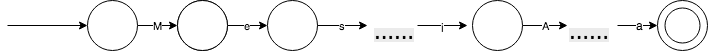
\includegraphics[scale=0.3]{img1}
\end{figure*}

$M_3$ accepts $L_1 \circ L_2$ $\Rightarrow$ $L_1 \circ L_2$ is regular.

\section{Non-determinism}

\begin{definition}
  A \underline{non-deterministic finite automaton} is a 5-tuple $M = (Q, \Sigma, \delta, q_0, F)$ s.t.
  \begin{itemize}
    \item $Q, \Sigma, q_0, F$ are the same
    \item $\delta: Q \times (\Sigma \cup \{\epsilon\}) \rightarrow 2^Q$
    \begin{itemize}
    \item $\delta (q, s)$ is a subset of $Q$
    \end{itemize} 
  \end{itemize}
\end{definition}

For a set $S$, $2^S$ is called the \underline{power set} of $S$. It contains all subsets of $S$.

$2^{\{a, b\}} = \{\emptyset, \{a\}, \{b\}, \{a, b\}\}$

\begin{definition}
  The NFA $M$ accepts the string  $w = w_1w_2 \cdots$if there exists a string $y = y_1y_2 \cdots y_m \in (\Sigma \cup \{\epsilon\})^*$  and a sequence $r0, r_1, \cdots r_m \in Q$ such that:
  \begin{itemize}
    \item $w = y_1 \circ y_2 \circ \cdots \circ y_m$
    \item $r_0 = q_0$
    \item $r_i \in \delta (r_{i-1}, y_i) \text{ for } i = 1, \cdots, m$
    \item $r_m \in F$
  \end{itemize}
\end{definition}

Input string: $w = 00$

$y = \epsilon 00$, $r = q_0q_1q_2q_1$

$\delta(q_0, \epsilon) = \{q_1, q_3\}$

\end{document}
